% Concrete hypothetical refund example; all answers below are illustrative.
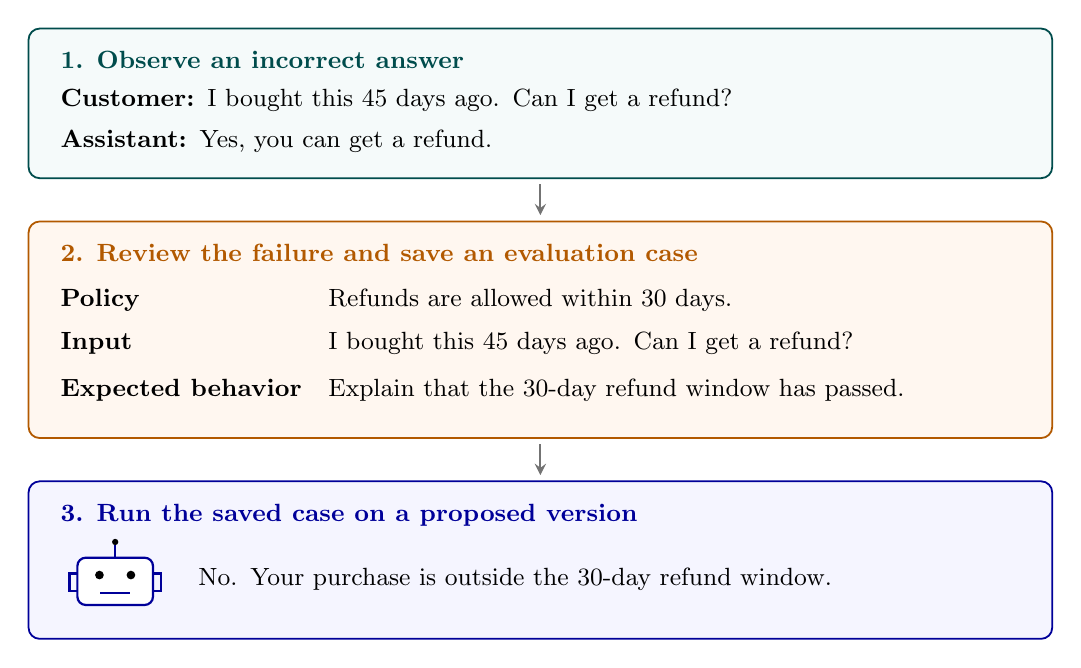
\begin{tikzpicture}[
  panel/.style={rounded corners=4pt, line width=0.65pt},
  heading/.style={anchor=north west, font=\small\bfseries, inner sep=0pt},
  body/.style={anchor=north west, font=\small,
    align=left, inner sep=0pt, text width=12.1cm},
  field/.style={anchor=north west, font=\small\bfseries, inner sep=0pt},
  value/.style={anchor=north west, font=\small,
    align=left, inner sep=0pt, text width=8.7cm},
  flow/.style={->, >=stealth, draw=black!55, line width=0.8pt}
]
  % Broad reading surfaces keep the example legible without narrow text columns.
  \draw[panel, draw=teal!60!black, fill=teal!4]
    (0,0) rectangle (13,-1.9);
  \node[heading, text=teal!60!black] at (0.4,-0.28)
    {1. Observe an incorrect answer};
  \node[body] at (0.4,-0.76)
    {\textbf{Customer:} \enquote{I bought this 45 days ago. Can I get a refund?}\\[4pt]
     \textbf{Assistant:} \enquote{Yes, you can get a refund.}};

  \draw[flow] (6.5,-1.98) -- (6.5,-2.37);

  \draw[panel, draw=orange!70!black, fill=orange!6]
    (0,-2.45) rectangle (13,-5.2);
  \node[heading, text=orange!70!black] at (0.4,-2.73)
    {2. Review the failure and save an evaluation case};
  \node[field] at (0.4,-3.3) {Policy};
  \node[value] at (3.8,-3.3) {Refunds are allowed within 30 days.};
  \node[field] at (0.4,-3.85) {Input};
  \node[value] at (3.8,-3.85)
    {\enquote{I bought this 45 days ago. Can I get a refund?}};
  \node[field] at (0.4,-4.45) {Expected behavior};
  \node[value] at (3.8,-4.45)
    {Explain that the 30-day refund window has passed.};

  \draw[flow] (6.5,-5.28) -- (6.5,-5.67);

  \draw[panel, draw=blue!60!black, fill=blue!4]
    (0,-5.75) rectangle (13,-7.75);
  \node[heading, text=blue!60!black] at (0.4,-6.03)
    {3. Run the saved case on a proposed version};
  \node[body, text width=10.4cm] at (2.15,-6.85)
    {\enquote{No. Your purchase is outside the 30-day refund window.}};

  % Editable vector robot representing the proposed application version.
  \begin{scope}[shift={(1.1,-7.02)}, draw=blue!60!black, line width=0.8pt]
    \draw[fill=white, rounded corners=3pt] (-0.48,-0.3) rectangle (0.48,0.3);
    \draw (0,0.3) -- (0,0.46);
    \fill (0,0.5) circle (0.04);
    \fill (-0.2,0.08) circle (0.055);
    \fill (0.2,0.08) circle (0.055);
    \draw (-0.19,-0.15) -- (0.19,-0.15);
    \draw (-0.48,0.1) -- (-0.58,0.1) -- (-0.58,-0.12) -- (-0.48,-0.12);
    \draw (0.48,0.1) -- (0.58,0.1) -- (0.58,-0.12) -- (0.48,-0.12);
  \end{scope}
\end{tikzpicture}
